\documentclass[14pt]{extbook}
\usepackage{multicol, enumerate, enumitem, hyperref, color, soul, setspace, parskip, fancyhdr} %General Packages
\usepackage{amssymb, amsthm, amsmath, latexsym, units, mathtools} %Math Packages
\everymath{\displaystyle} %All math in Display Style
% Packages with additional options
\usepackage[headsep=0.5cm,headheight=12pt, left=1 in,right= 1 in,top= 1 in,bottom= 1 in]{geometry}
\usepackage[usenames,dvipsnames]{xcolor}
\usepackage{dashrule}  % Package to use the command below to create lines between items
\newcommand{\litem}[1]{\item#1\hspace*{-1cm}\rule{\textwidth}{0.4pt}}
\pagestyle{fancy}
\lhead{Makeup Progress Quiz 3}
\chead{}
\rhead{Version C}
\lfoot{1648-1753}
\cfoot{}
\rfoot{Summer C 2021}
\begin{document}

\begin{enumerate}
\litem{
Choose the equation of the function graphed below.
\begin{center}
    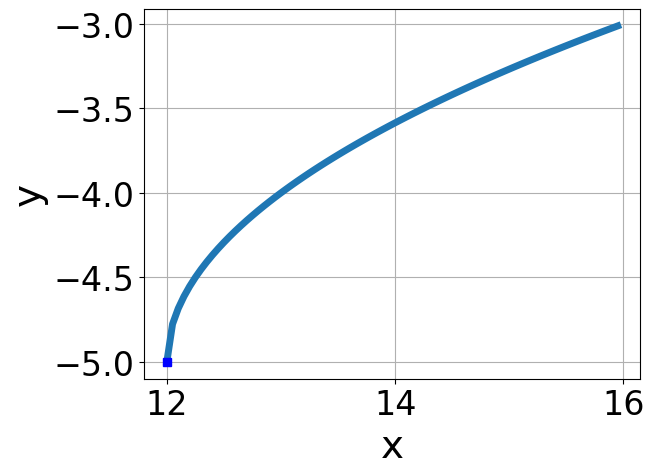
\includegraphics[width=0.5\textwidth]{../Figures/radicalGraphToEquationC.png}
\end{center}
\begin{enumerate}[label=\Alph*.]
\item \( f(x) = - \sqrt[3]{x - 12} - 5 \)
\item \( f(x) = \sqrt[3]{x - 12} - 5 \)
\item \( f(x) = - \sqrt[3]{x + 12} - 5 \)
\item \( f(x) = \sqrt[3]{x + 12} - 5 \)
\item \( \text{None of the above} \)

\end{enumerate} }
\litem{
Choose the graph of the equation below.\[ f(x) = - \sqrt[3]{x + 12} + 3 \]\begin{enumerate}[label=\Alph*.]
\begin{multicols}{2}\item 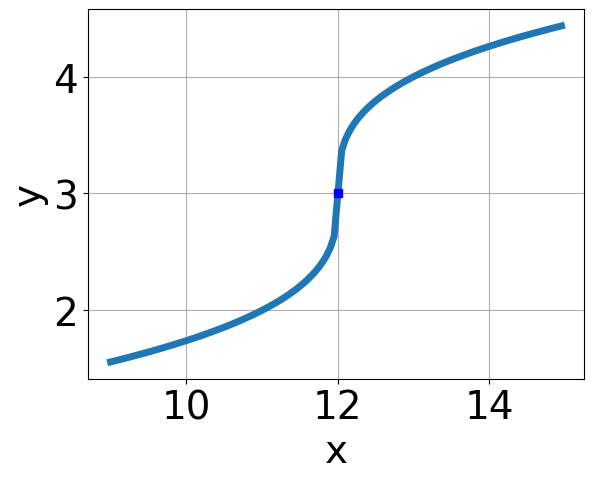
\includegraphics[width = 0.3\textwidth]{../Figures/radicalEquationToGraphCopyAC.png}\item 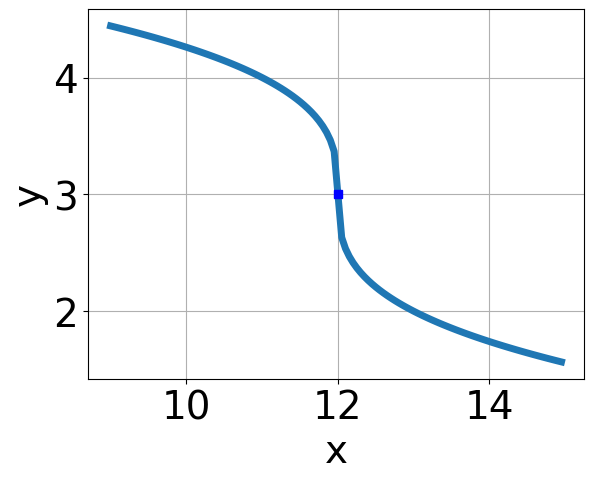
\includegraphics[width = 0.3\textwidth]{../Figures/radicalEquationToGraphCopyBC.png}\item 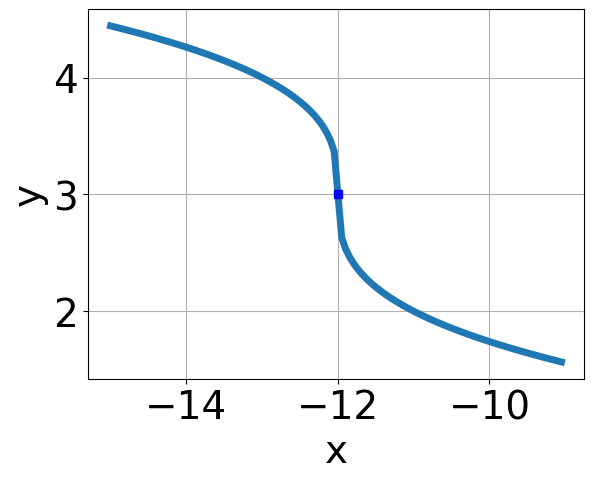
\includegraphics[width = 0.3\textwidth]{../Figures/radicalEquationToGraphCopyCC.png}\item 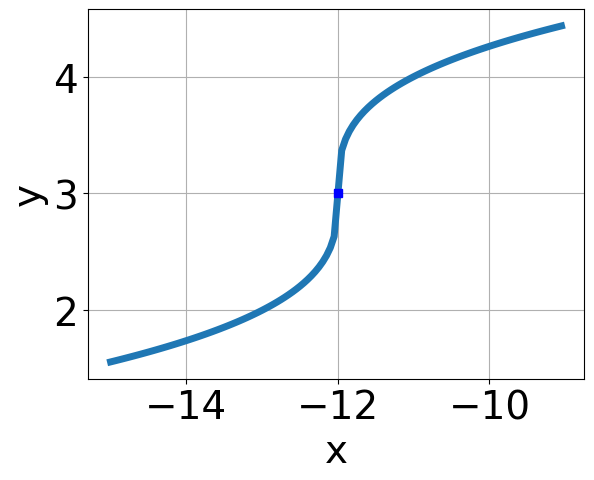
\includegraphics[width = 0.3\textwidth]{../Figures/radicalEquationToGraphCopyDC.png}\end{multicols}\item None of the above.
\end{enumerate} }
\litem{
What is the domain of the function below?\[ f(x) = \sqrt[4]{-4 x - 5} \]\begin{enumerate}[label=\Alph*.]
\item \( [a, \infty), \text{where } a \in [-2.36, -0.83] \)
\item \( (-\infty, \infty) \)
\item \( (-\infty, a], \text{where } a \in [-0.93, -0.64] \)
\item \( (-\infty, a], \text{ where } a \in [-1.43, -0.91] \)
\item \( [a, \infty), \text{where } a \in [-1.11, 1.51] \)

\end{enumerate} }
\litem{
Solve the radical equation below. Then, choose the interval(s) that the solution(s) belongs to.\[ \sqrt{12 x^2 - 14} - \sqrt{38 x} = 0 \]\begin{enumerate}[label=\Alph*.]
\item \( x_1 \in [-0.29, 0.48] \text{ and } x_2 \in [3.5,5.5] \)
\item \( x \in [-0.57,0.19] \)
\item \( x \in [2.68,4.7] \)
\item \( \text{All solutions lead to invalid or complex values in the equation.} \)
\item \( x_1 \in [-0.57, 0.19] \text{ and } x_2 \in [3.5,5.5] \)

\end{enumerate} }
\litem{
Choose the equation of the function graphed below.
\begin{center}
    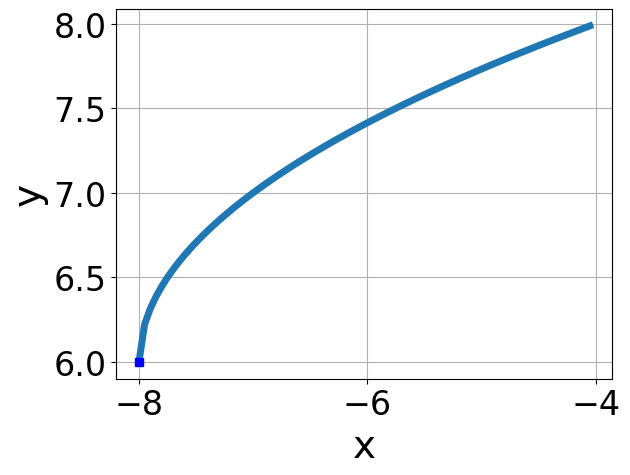
\includegraphics[width=0.5\textwidth]{../Figures/radicalGraphToEquationCopyC.png}
\end{center}
\begin{enumerate}[label=\Alph*.]
\item \( f(x) = - \sqrt{x + 8} + 6 \)
\item \( f(x) = - \sqrt{x - 8} + 6 \)
\item \( f(x) = \sqrt{x - 8} + 6 \)
\item \( f(x) = \sqrt{x + 8} + 6 \)
\item \( \text{None of the above} \)

\end{enumerate} }
\litem{
Solve the radical equation below. Then, choose the interval(s) that the solution(s) belongs to.\[ \sqrt{5 x - 4} - \sqrt{-7 x + 9} = 0 \]\begin{enumerate}[label=\Alph*.]
\item \( x_1 \in [0.78, 0.91] \text{ and } x_2 \in [1.25,1.29] \)
\item \( x_1 \in [0.78, 0.91] \text{ and } x_2 \in [0.84,1.12] \)
\item \( x \in [-0.61,-0.31] \)
\item \( x \in [0.97,1.1] \)
\item \( \text{All solutions lead to invalid or complex values in the equation.} \)

\end{enumerate} }
\litem{
Solve the radical equation below. Then, choose the interval(s) that the solution(s) belongs to.\[ \sqrt{-35 x^2 + 36} - \sqrt{-43 x} = 0 \]\begin{enumerate}[label=\Alph*.]
\item \( \text{All solutions lead to invalid or complex values in the equation.} \)
\item \( x_1 \in [0, 1.05] \text{ and } x_2 \in [-0.2,2.8] \)
\item \( x_1 \in [-1.1, -0.09] \text{ and } x_2 \in [-0.2,2.8] \)
\item \( x \in [-1.1,-0.09] \)
\item \( x \in [1.33,2.34] \)

\end{enumerate} }
\litem{
Solve the radical equation below. Then, choose the interval(s) that the solution(s) belongs to.\[ \sqrt{-4 x - 9} - \sqrt{-5 x + 7} = 0 \]\begin{enumerate}[label=\Alph*.]
\item \( x \in [15,17] \)
\item \( x_1 \in [-7.25, 0.75] \text{ and } x_2 \in [15,17] \)
\item \( \text{All solutions lead to invalid or complex values in the equation.} \)
\item \( x \in [1,4] \)
\item \( x_1 \in [-7.25, 0.75] \text{ and } x_2 \in [0.4,6.4] \)

\end{enumerate} }
\litem{
Choose the graph of the equation below.\[ f(x) = - \sqrt[3]{x + 10} + 7 \]\begin{enumerate}[label=\Alph*.]
\begin{multicols}{2}\item 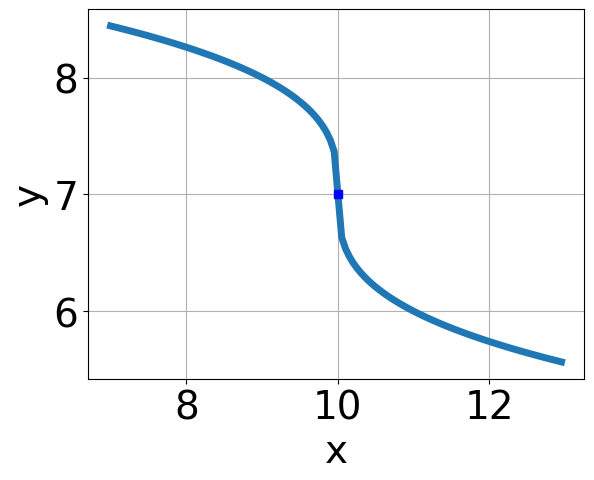
\includegraphics[width = 0.3\textwidth]{../Figures/radicalEquationToGraphAC.png}\item 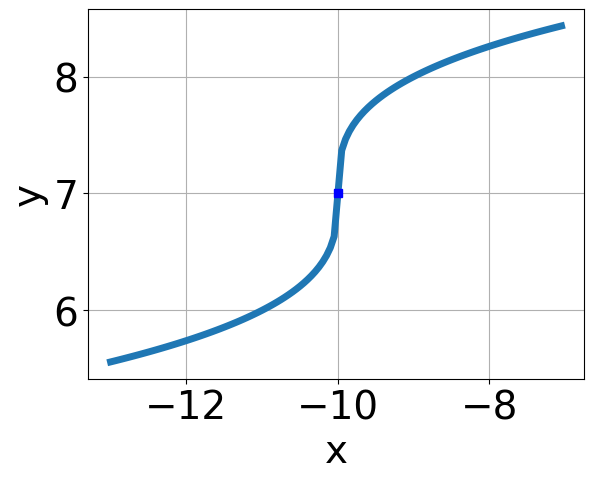
\includegraphics[width = 0.3\textwidth]{../Figures/radicalEquationToGraphBC.png}\item 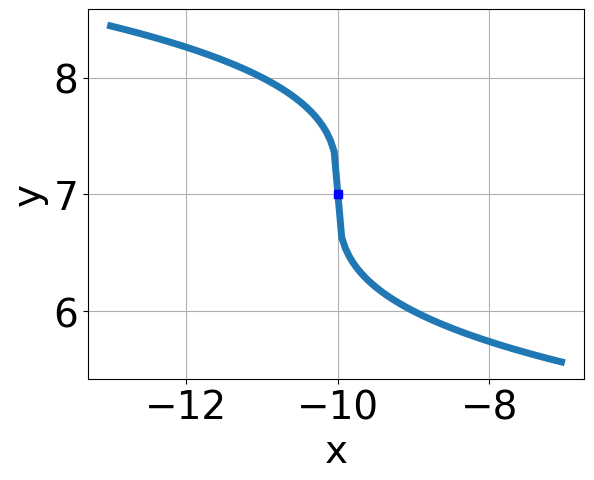
\includegraphics[width = 0.3\textwidth]{../Figures/radicalEquationToGraphCC.png}\item 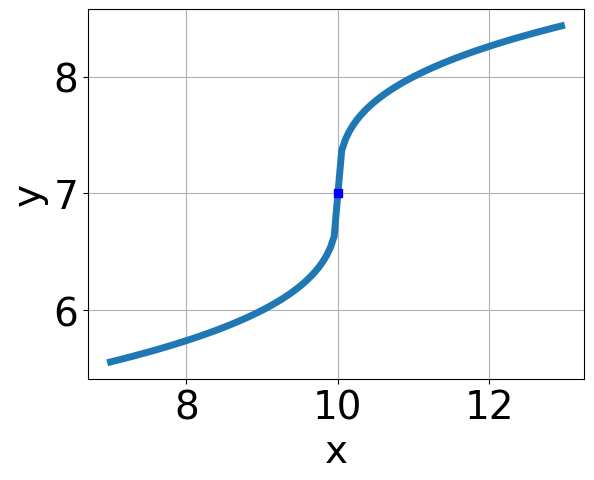
\includegraphics[width = 0.3\textwidth]{../Figures/radicalEquationToGraphDC.png}\end{multicols}\item None of the above.
\end{enumerate} }
\litem{
What is the domain of the function below?\[ f(x) = \sqrt[4]{-6 x - 5} \]\begin{enumerate}[label=\Alph*.]
\item \( [a, \infty), \text{where } a \in [-0.85, -0.18] \)
\item \( (-\infty, \infty) \)
\item \( (-\infty, a], \text{where } a \in [-1.94, -0.87] \)
\item \( [a, \infty), \text{where } a \in [-1.76, -1.11] \)
\item \( (-\infty, a], \text{ where } a \in [-0.98, -0.42] \)

\end{enumerate} }
\end{enumerate}

\end{document}